\documentclass[10pt]{homeworg}

\usepackage{bm}
\title{Homework 3}
\author{Kevin Yang - 50244152}


\begin{document}

\maketitle

\Huge{Link to repo:}\\
\Large{https://github.com/keviny2/CPSC532W-Assignments/tree/main/FOPPL}


\section{Program 1}
\begin{center}
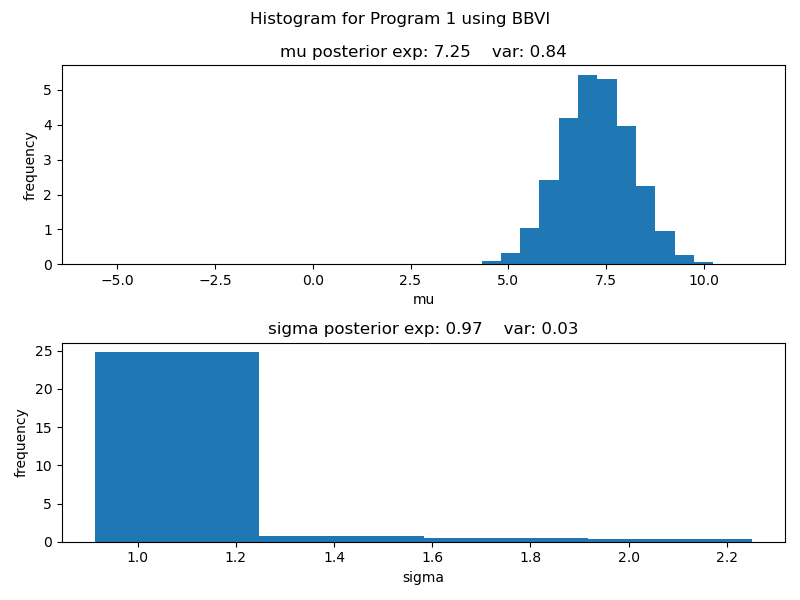
\includegraphics[scale=0.5]{figures/BBVI_program_1.png}
\end{center}

\begin{figure}
    \centering
    \begin{minipage}{0.45\textwidth}
        \centering
       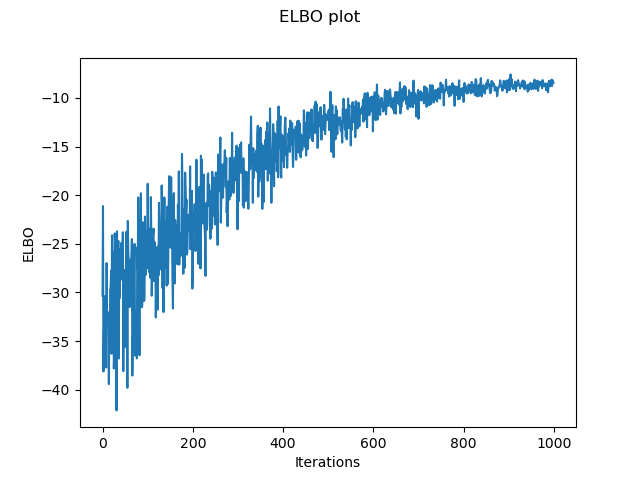
\includegraphics[scale=0.5]{figures/elbo_program_1.png}
    \end{minipage}\hfill
    \begin{minipage}{0.45\textwidth}
        \centering
        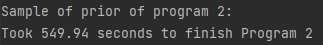
\includegraphics[scale=0.8]{figures/program1_time.png}
    \end{minipage}
\end{figure}

\newpage

%%%%%%%%%%%%%%%%%%%%%%%%%%%%%%%%%%%%%%%%%%%%%%%%%%%%%%

\section{Program 2}
\begin{center}
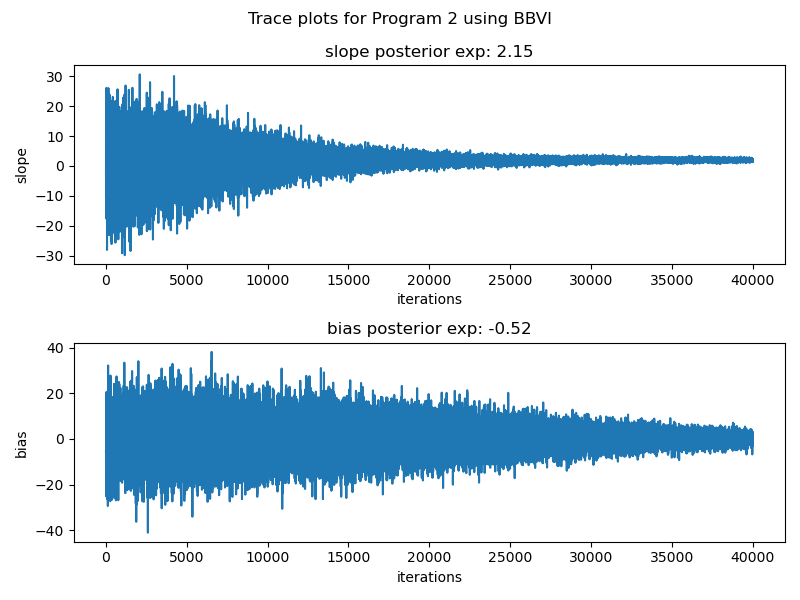
\includegraphics[scale=0.5]{figures/BBVI_program_2.png}
\end{center}

\begin{figure}[!htbp]
    \centering
    \begin{minipage}{0.45\textwidth}
        \centering
       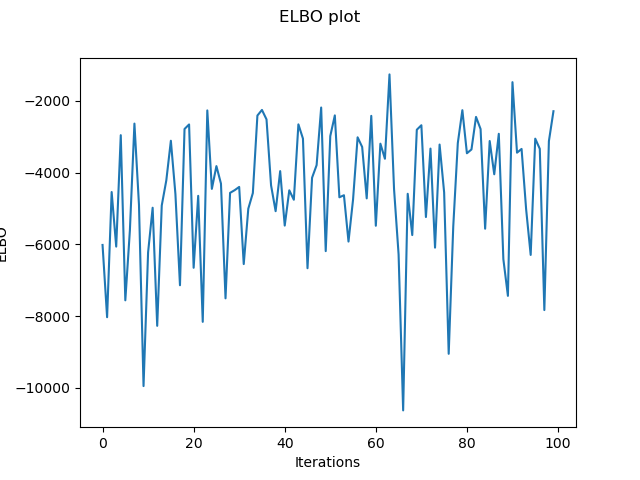
\includegraphics[scale=0.5]{figures/elbo_program_2.png}
    \end{minipage}\hfill
    \begin{minipage}{0.45\textwidth}
        \centering
        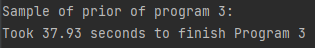
\includegraphics[scale=0.8]{figures/program2_time.png}
    \end{minipage}
\end{figure}


%%%%%%%%%%%%%%%%%%%%%%%%%%%%%%%%%%%%%%%%%%%%%%%%%%%%%%

\section{Program 3}


%%%%%%%%%%%%%%%%%%%%%%%%%%%%%%%%%%%%%%%%%%%%%%%%%%%%%%

\section{Program 4}
\begin{figure}[!htbp]
    \centering
    \begin{minipage}{0.45\textwidth}
        \centering
       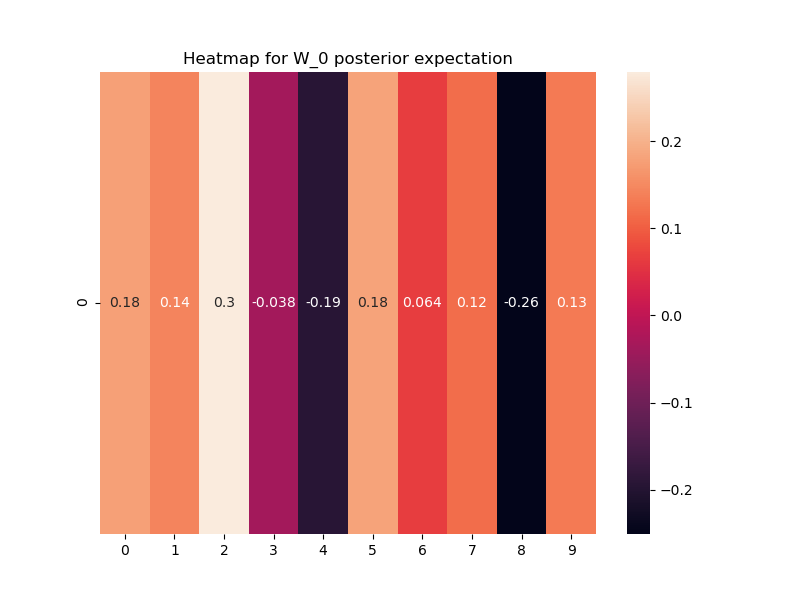
\includegraphics[scale=0.5]{figures/heatmap_exp_W_0.png}
    \end{minipage}\hfill
    \begin{minipage}{0.45\textwidth}
        \centering
        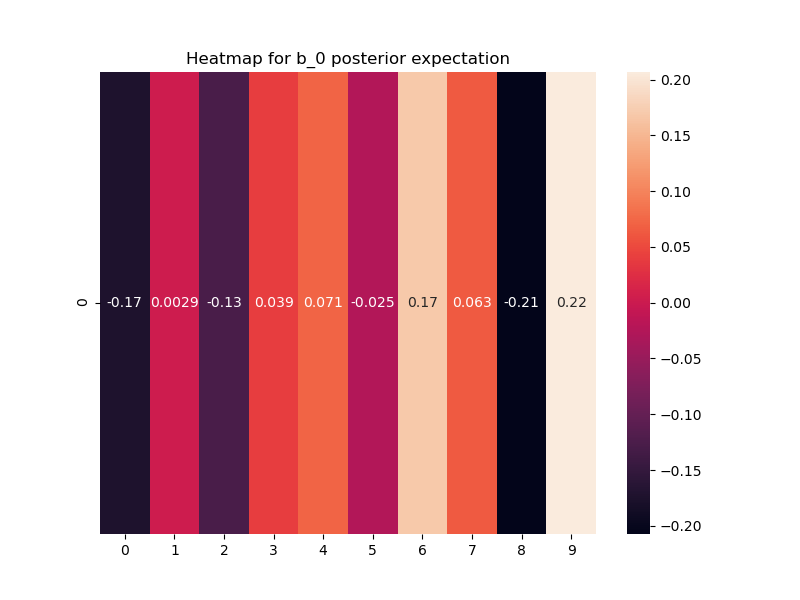
\includegraphics[scale=0.5]{figures/heatmap_exp_b_0.png}
    \end{minipage}
\end{figure}

\begin{figure}[!htbp]
    \centering
    \begin{minipage}{0.45\textwidth}
        \centering
       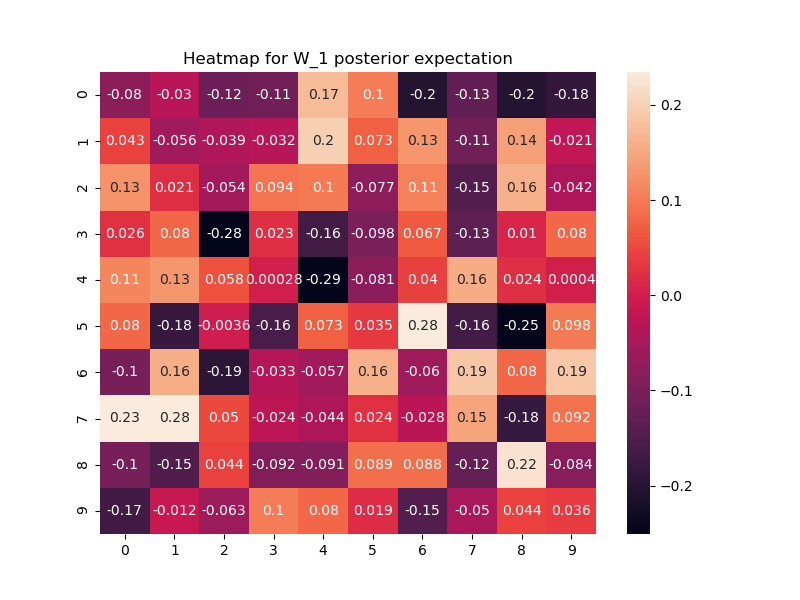
\includegraphics[scale=0.5]{figures/heatmap_exp_W_1.png}
    \end{minipage}\hfill
    \begin{minipage}{0.45\textwidth}
        \centering
        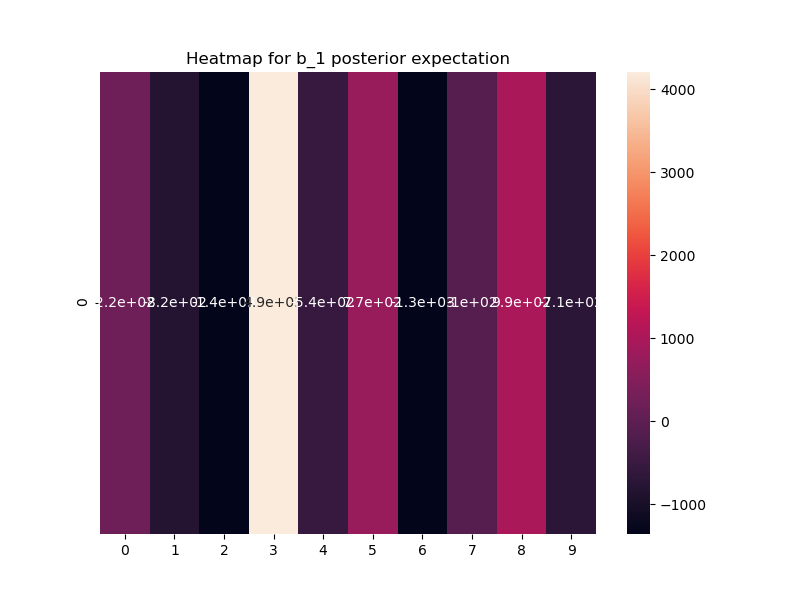
\includegraphics[scale=0.5]{figures/heatmap_exp_b_1.png}
    \end{minipage}
\end{figure}

\begin{figure}[!htbp]
    \centering
    \begin{minipage}{0.45\textwidth}
        \centering
       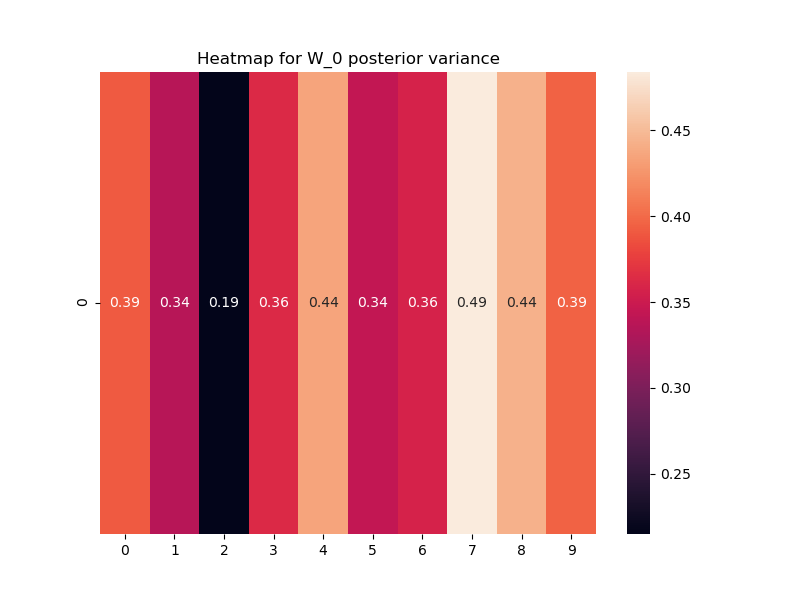
\includegraphics[scale=0.5]{figures/heatmap_var_W_0.png}
    \end{minipage}\hfill
    \begin{minipage}{0.45\textwidth}
        \centering
        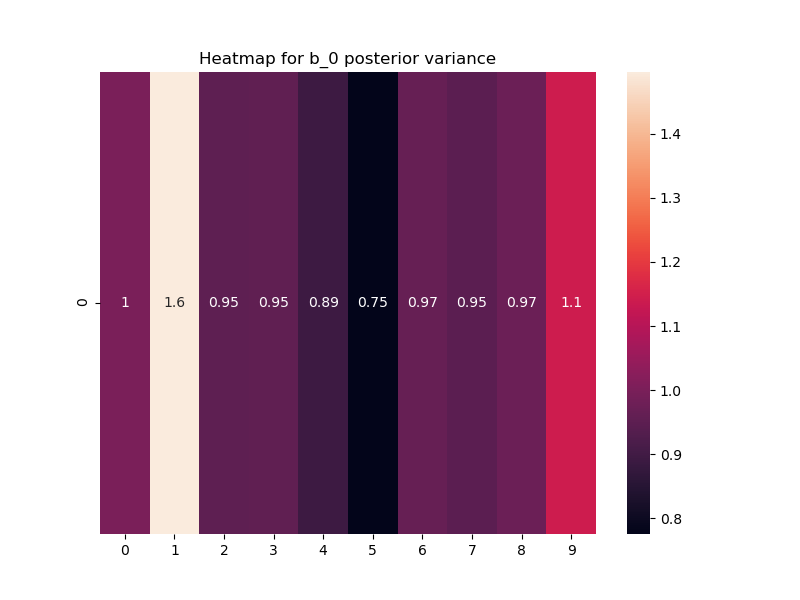
\includegraphics[scale=0.5]{figures/heatmap_var_b_0.png}
    \end{minipage}
\end{figure}

\begin{figure}[!htbp]
    \centering
    \begin{minipage}{0.45\textwidth}
        \centering
       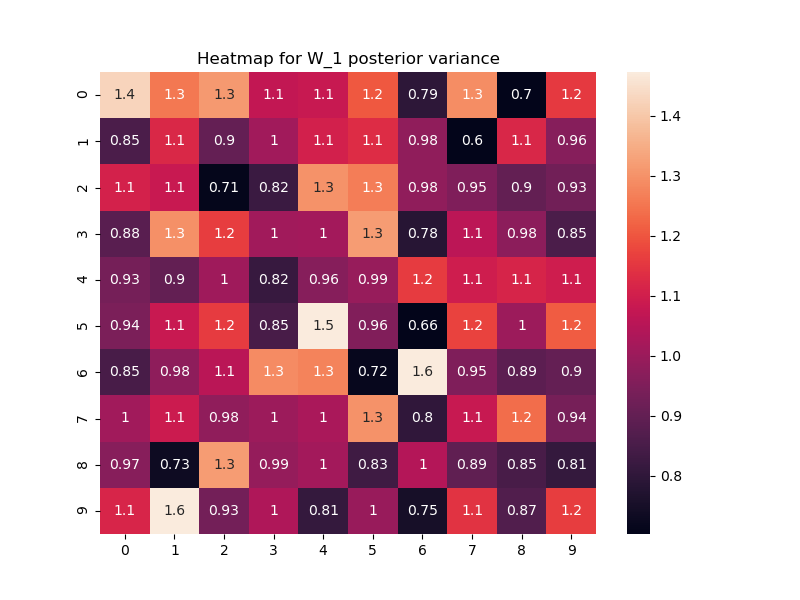
\includegraphics[scale=0.5]{figures/heatmap_var_W_1.png}
    \end{minipage}\hfill
    \begin{minipage}{0.45\textwidth}
        \centering
        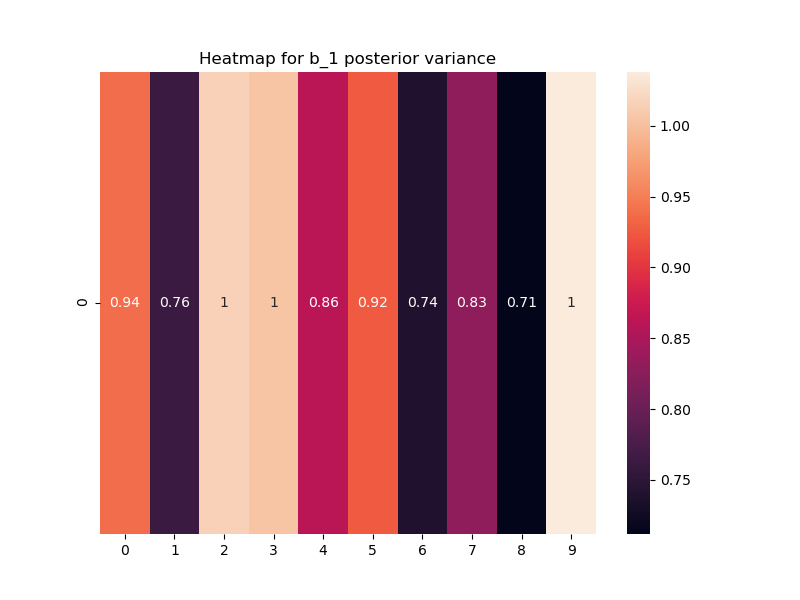
\includegraphics[scale=0.5]{figures/heatmap_var_b_1.png}
    \end{minipage}
\end{figure}

\begin{figure}[!htbp]
    \centering
    \begin{minipage}{0.45\textwidth}
        \centering
       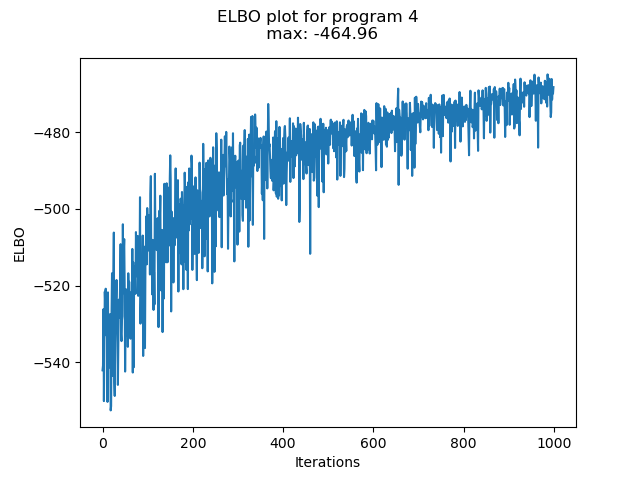
\includegraphics[scale=0.5]{figures/elbo_program_4.png}
    \end{minipage}\hfill
    \begin{minipage}{0.45\textwidth}
        \centering
        
\includegraphics[scale=0.8]{figures/program4_time.png}
    \end{minipage}
\end{figure}


Black-box variational inference (BBVI) is more generic compared to parameter estimation via gradient descent. In BBVI, we compute an estimate of the gradient of the evidence lower bound (ELBO) using a sampling procedure instead of obtaining the gradient of the ELBO analytically. This renders BBVI applicable to a range of complicated models that parameter estimation via gradient descent will not be able to handle.

%%%%%%%%%%%%%%%%%%%%%%%%%%%%%%%%%%%%%%%%%%%%%%%%%%%%%%

\section{Program 5}


\end{document}